\begin{frame}
  \begin{tikzpicture}
    \begin{axis}[ xbar=0pt, /pgf/bar shift=0pt, legend style={ legend columns=4,
        at={(xticklabel cs:0.5)}, anchor=north, draw=none }, ytick={0,...,15},
      ytick style={draw=none},% <- added
      axis y line*=none, axis x line*=bottom, tick label
      style={font=\footnotesize}, legend style={font=\footnotesize}, label
      style={font=\footnotesize}, xtick style={draw=none},% <- added
      xtick={0,1,...,12}, width=.9\textwidth, bar width=3mm, y dir = reverse,
      xmin=0, xmax=13, area legend,
      y=5mm, enlarge y limits={abs=0.625},
      style={text=black}, every axis plot/.append style={fill},
      nodes near coords, nodes near coords,
      yticklabels={%
        {\topicref{Grenseverdier}},
        {\topicref{Gradient}},
        {\topicref{Epsilon-delta}},
        {\topicref{Kjerneregelen}},
        {\topicref{Taylor-approksimasjon}},
        {\topicref{Tangenter}},
        {\topicref{Kritiske-punkter}},
        {\topicref{Optimering}},
        {\topicref{Linjeintegral}},
        {\topicref{Konservative-vektorfelt}},
        {\topicref{Dobbelintegraler}},
        {\topicref{Integrasjonsrekkefolge}},
        {\topicref{Trippelintegral}},
        {\topicref{Greens-teorem}},
        {\topicref{Divergensteoremet}},
        {\topicref{Stokes-teorem}}}]
      \addplot[fill=gray] coordinates {(8,0)};
      \addplot[fill=gray] coordinates {(4,1)};
      \addplot[fill=gray] coordinates {(1,2)};
      \addplot[fill=gray] coordinates {(7,3)};
      \addplot[fill=gray] coordinates {(1,4)};
      \addplot[fill=gray] coordinates {(7,5)};
      \addplot[fill=gray] coordinates {(11,6)};
      \addplot[fill=dgreen] coordinates {(4,7)};
      \addplot[fill=black] coordinates {(3,8)};
      \addplot[fill=black] coordinates {(8,9)};
      \addplot[fill=black] coordinates {(7,10)};
      \addplot[fill=black] coordinates {(3,11)};
      \addplot[fill=black] coordinates {(4,12)};
      \addplot[fill=black] coordinates {(4,13)};
      \addplot[fill=black] coordinates {(8,14)};
      \addplot[fill=black] coordinates {(6,15)};
    \end{axis}
  \end{tikzpicture}
\end{frame}

\begin{frame}
  \subsection{Optimering}\label{subsec:Optimering}
  \frametitle{Optimering}
  \begin{oppgave}{K2015, Oppgave 4a}
    Finn punktene på kuleflaten $x^2 + y^2 + z^2 = 4$ som er nærmeste og lengst
    fra punktet $(2,2,1)$.
  \end{oppgave}%
  \visible<1->{
    \only<1-3>{
    Avstanden mellom punktet $(x,y,z)$ og $(2,2,1)$ er
    %
    \begin{equation*}
      f(x,y,z) = (x-2)^2 + (y-2)^2 + (z-1)^2
    \end{equation*}
    %
    Vi ønsker å optimalisere denne avstanden under bi-bibetingelsen
    om at punktet vårt ligger på kuleflaten. Altså $g(x,y,z)=x^2+y^2+z^2-4$.
    %
    \begin{equation*}
      \nabla f = \lambda \nabla g
      \Leftrightarrow 2(x - 2, y - 2, z - 1) = 2 \lambda (x,y,z)
    \end{equation*}
    %
    \only<2>{
    Her har vi altså tre likninger med tre ukjente. Med løsning
    %
    \begin{equation*}
      x = \frac{2}{1 - \lambda} = y \quad \text{og} \quad z = \frac{1}{1-\lambda}
  \end{equation*}}
  \only<3>{ Innsatt i $g(x,y,z)$ får vi da
    \begin{equation*}
      \Bigl(\frac{1}{1-\lambda}\Bigr)^2(2^2 + 2^2 + 1) = 4
      \Rightarrow \frac{1}{1-\lambda} = \pm \frac{2}{3}
  \end{equation*}
  %
  slik at $x=y=\pm 4/3$, $z=\pm 2/3$ punktene $(4,4,2)/3$ og $(-4,-4,-2)/3$
  som
}}
\only<4-5>{
\begin{columns}[T] % align columns
\begin{column}{.47\textwidth}
  \visible<4-5>{
For å reise raskest mulig bort fra kulen
må vi reise normalt bort fra den. Dette
er retningen til normalvektoren
$\vek{n}=(2,2,1)$.
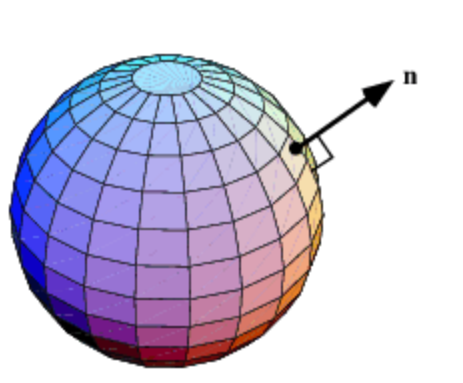
\includegraphics[width=0.75\textwidth]{normalvektor.png}}
\end{column}%
\hfill%
\begin{column}{.50\textwidth}
  \visible<5>{
  Finner skjæringspunktet mellom
  %
  \begin{equation*}
    \ell(t) = (0,0,0)+t(2,2,1) = t(2,2,1)
  \end{equation*}
  %
  og kuleflaten $x^2+y^2+z^2=4$. Dette gir
  %
  \begin{equation*}
    (2t)^2+  (2t)^2 + (t)^2 = 4
    \Rightarrow t = \pm \frac{2}{3}
  \end{equation*}
  %
  Leser kan selv teste at en får samme punkter
ved å sette $t$ inn i $\ell$.}
\end{column}%
\end{columns}
}
  }
\end{frame}

